\providecommand{\main}{../../../..}
\documentclass[\main/dresen_thesis.tex]{subfiles}
\begin{document}
  \label{sec:looselyPackedNS:nanoparticle:vsm}

  To study the magnetic structure of the nanoparticles, vibrating sample magnetometry (VSM) is applied to measure the macroscopic magnetization of a dispersion as described in \refapp{app:additionalExperimentalTechniques:vsm} and polarized small-angle neutron scattering (SANSPOL) is applied to measure the magnetic scattering of the individual nanoparticles.
  Both techniques allow to model the average individual nanoparticle magnetization and the results should be in agreement with one another.

  For SANSPOL, a magnetic field of $B\eq 515 \unit{mT}$ was applied perpendicular \& horizontal to the beam direction and the scattered neutrons are counted on a position-sensitive detector for up and down polarized neutrons without polarization analysis after the scattering.
  The same model and parameters as obtained from the nuclear small-angle scattering is used and extended by a spherical magnetic form factor.
  The magnetic SLD of the core is fitted as parameter and possibly it is allowed that the magnetic radius of the particle is smaller by a size of $d_\mathrm{dead}$ due to a magnetically dead surface layer.
  From the magnetic SLD, the volume magnetization is calculated using \refeq{eq:theoreticalBackground:scattering:magneticSLD}
  \begin{align}
    \label{eq:looselyPackedNP:nanoparticles:SLDtoMagnetization}
    M \eq& \mu_B s_e \eq \frac{2 \pi \hbar^2}{m_n \mu_0 \mu_n} \rho_\mathrm{mag},\\
    \frac{M}{\bigg[\unit{kA m^{-1}}\bigg]} \eq& 343.592 \cdot \frac{\rho_\mathrm{mag}}{\bigg[10^{-6} \angstrom^{-2} \bigg]}.
  \end{align}
  The obtained model is shown in \reffig{fig:looselyPackedNP:nanoparticle:sanspol} and the results in \reftab{tab:looselyPackedNP:nanoparticle:vsmSanspol}.

  \begin{figure}[tb]
    \centering
    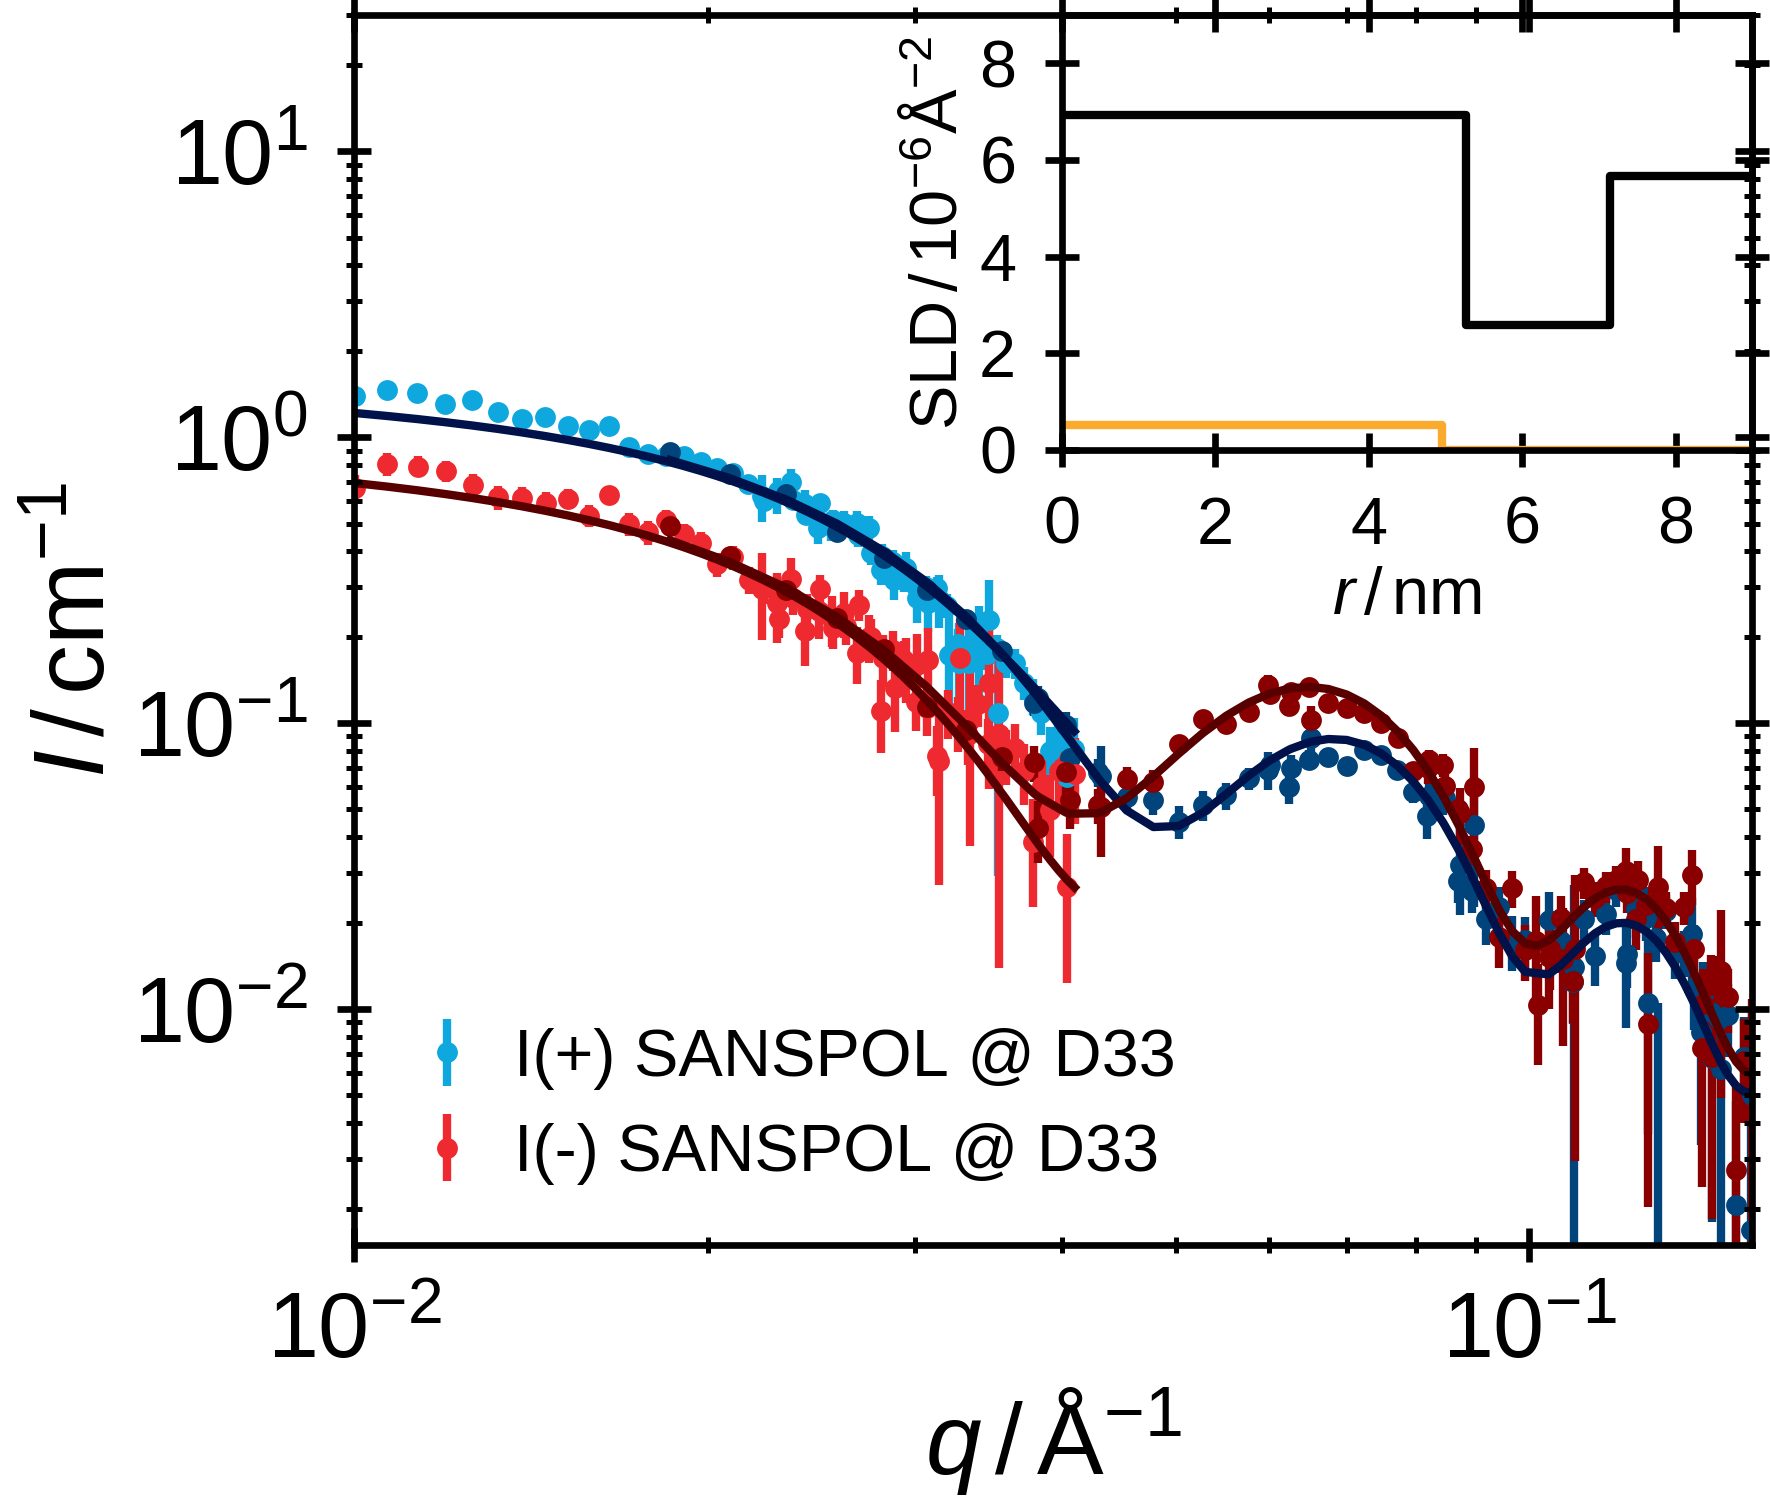
\includegraphics{looselyPackedNP_SAS_IOS-11_SANSPOLFit}
    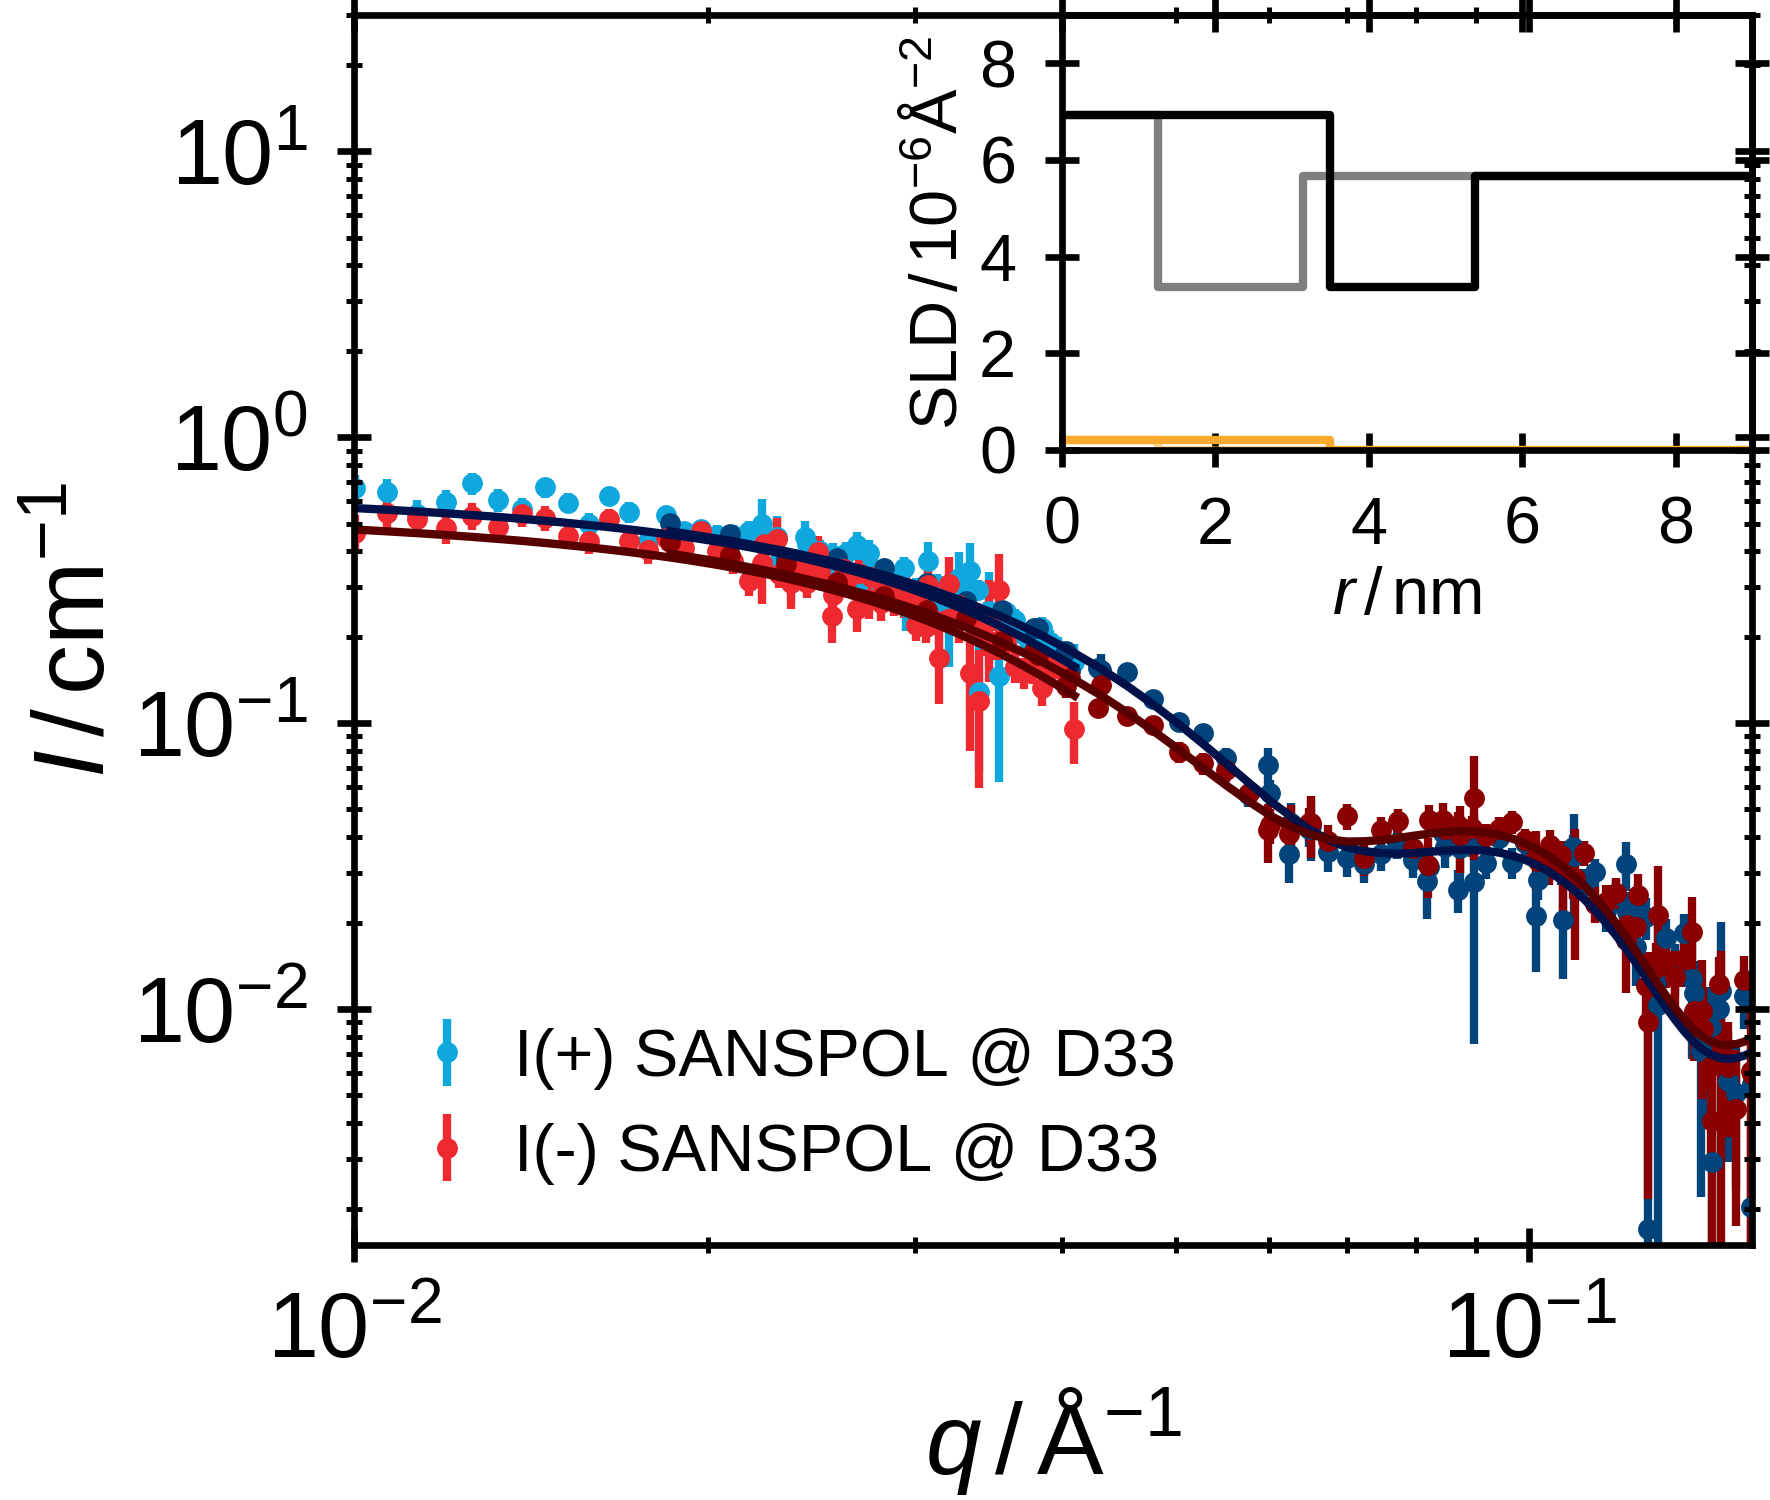
\includegraphics{looselyPackedNP_SAS_IOS-7_SANSPOLFit}
    \caption{\label{fig:looselyPackedNP:nanoparticle:sanspol}Polarized small-angle neutron scattering for IOS-11 (left) and IOS-7 (right).}
  \end{figure}


  For the VSM data, it is assumed that the dispersion is compromised of homogeneously magnetized, non-interacting particles that can be represented by a single classical super spin.
  In \refapp{ch:appendix:calculations:magnetizationClassicalSpin}, it is shown that in this case the magnetization is given by a Langevin curve
  \begin{align}
    M(H) \eq& M_s \biggl( \coth \biggl(\frac{\mu \mu_0 H}{k_B T} \biggr) - \frac{k_B T}{\mu \mu_0 H} \biggr) + \chi H.
  \end{align}
  Here, $M_s$ is the saturation magnetization, $\mu$ the magnetic moment of one nanoparticle and $\chi$ the excess susceptibility.
  To properly obtain the saturation magnetization in units of $\unit{kAm{-1}}$, the exact volume of magnetic material in dispersion needs to be known and the measured magnetization data scaled accordingly.
  The volume of the magnetic material can be estimated either by gravimetric methods or also by using the results obtained from small-angle scattering.
  As one parameter in the small-angle scattering model is the number of particles per volume $n \eq N/V$ and another the volume of the particle $V_p$, the magnetic volume per dispersion volume is given by
  \begin{align}
    \alpha \eq \frac{N V_p}{V}.
  \end{align}
  This ratio is multiplied with the volume of dispersion measured in the VSM experiment to obtain the volume that the final data is scaled to.
  The data and best-fit model are shown in \reffig{fig:looselyPackedNP:nanoparticle:vsm} and the numerical values are given in \reftab{tab:looselyPackedNP:nanoparticle:vsmSanspol}.

  \begin{figure}[tb]
    \centering
    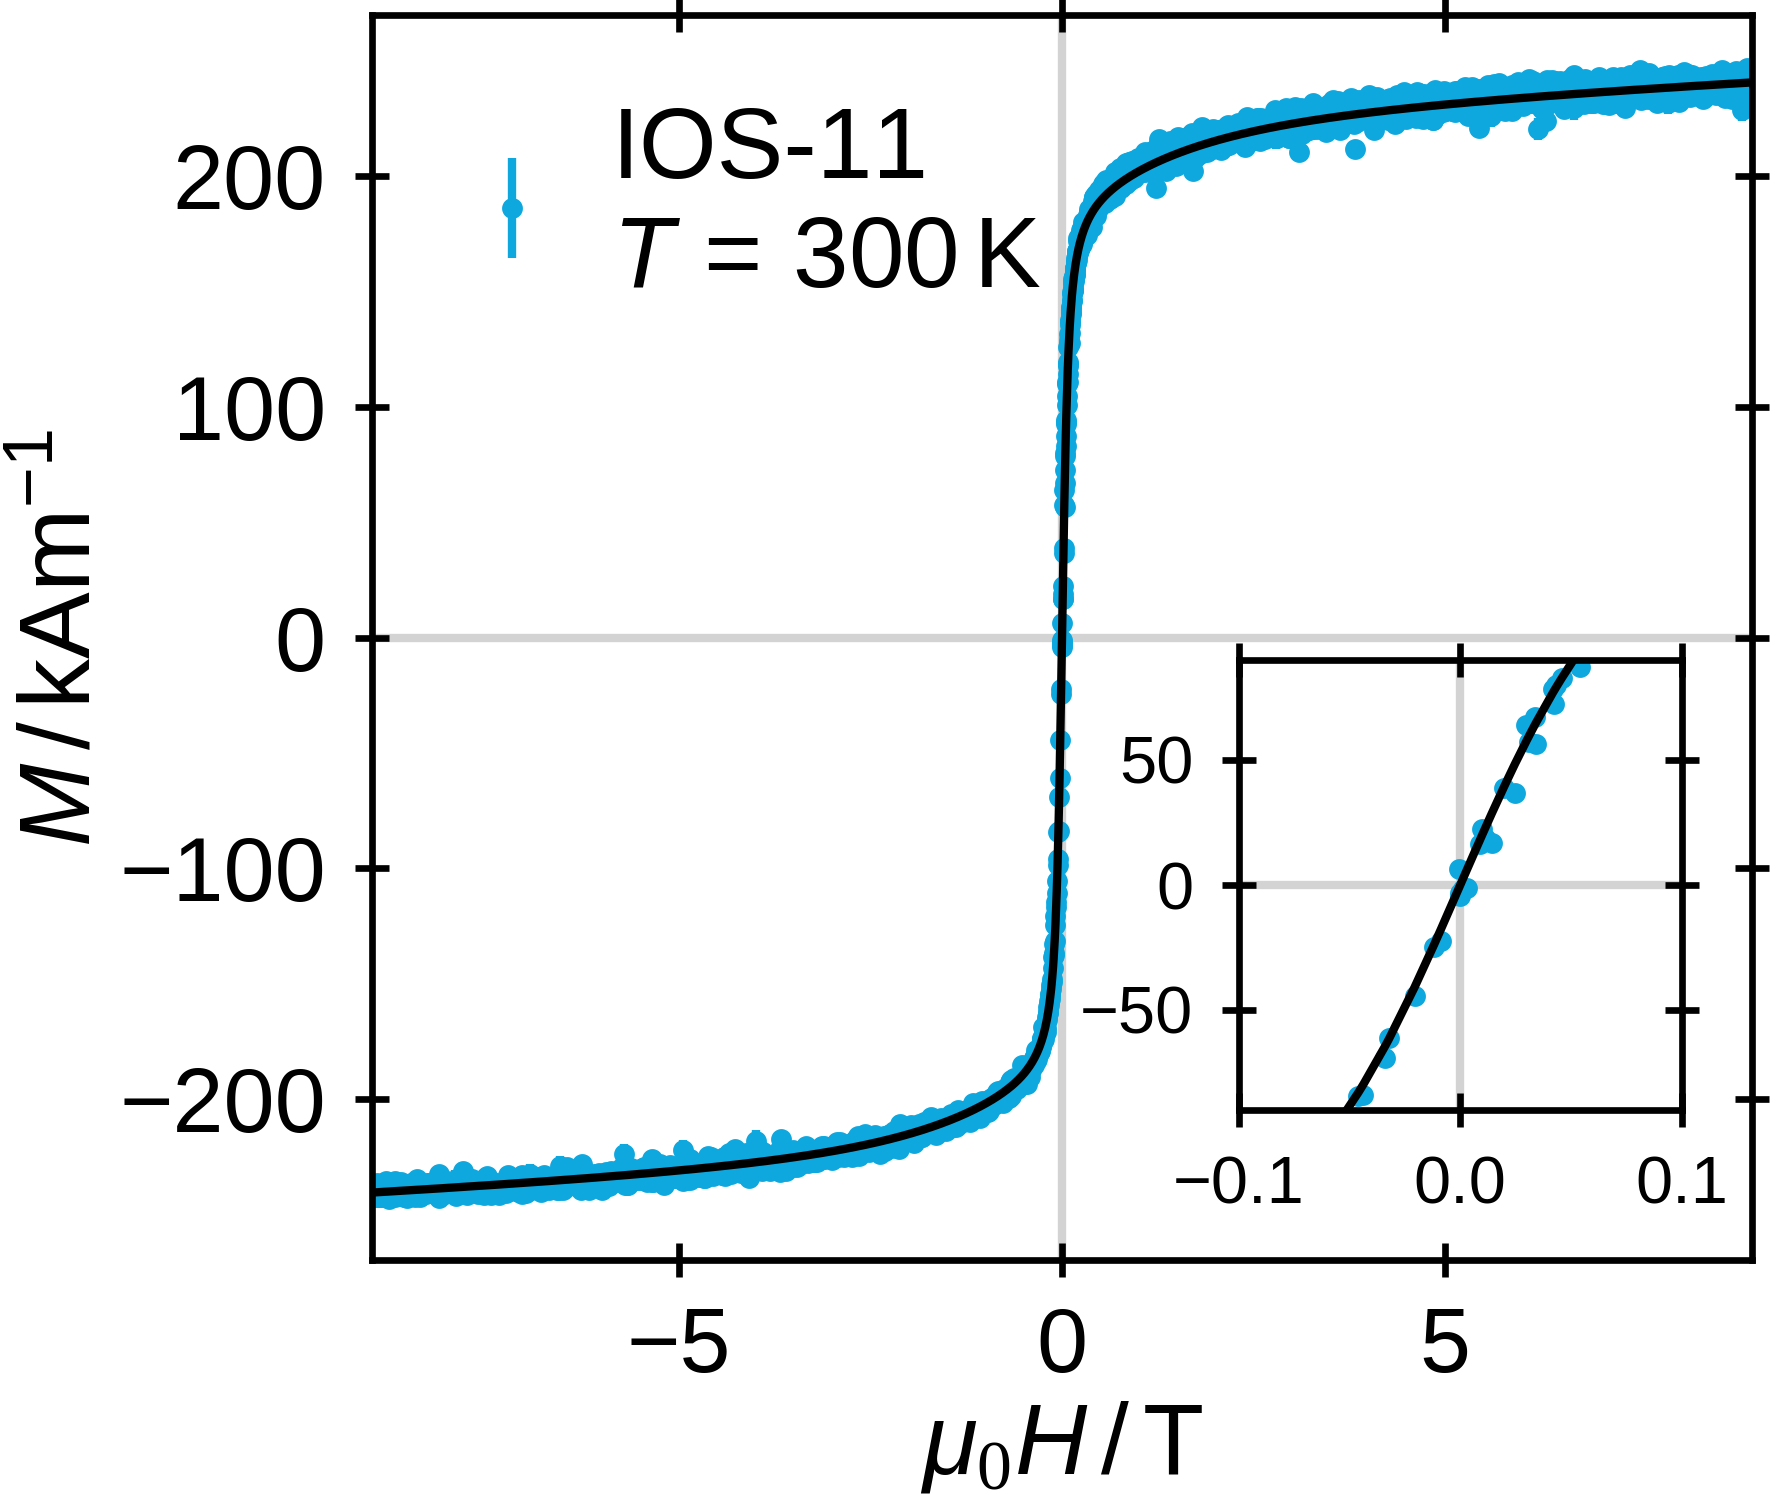
\includegraphics{looselyPackedNP_VSM_IOS-11}
    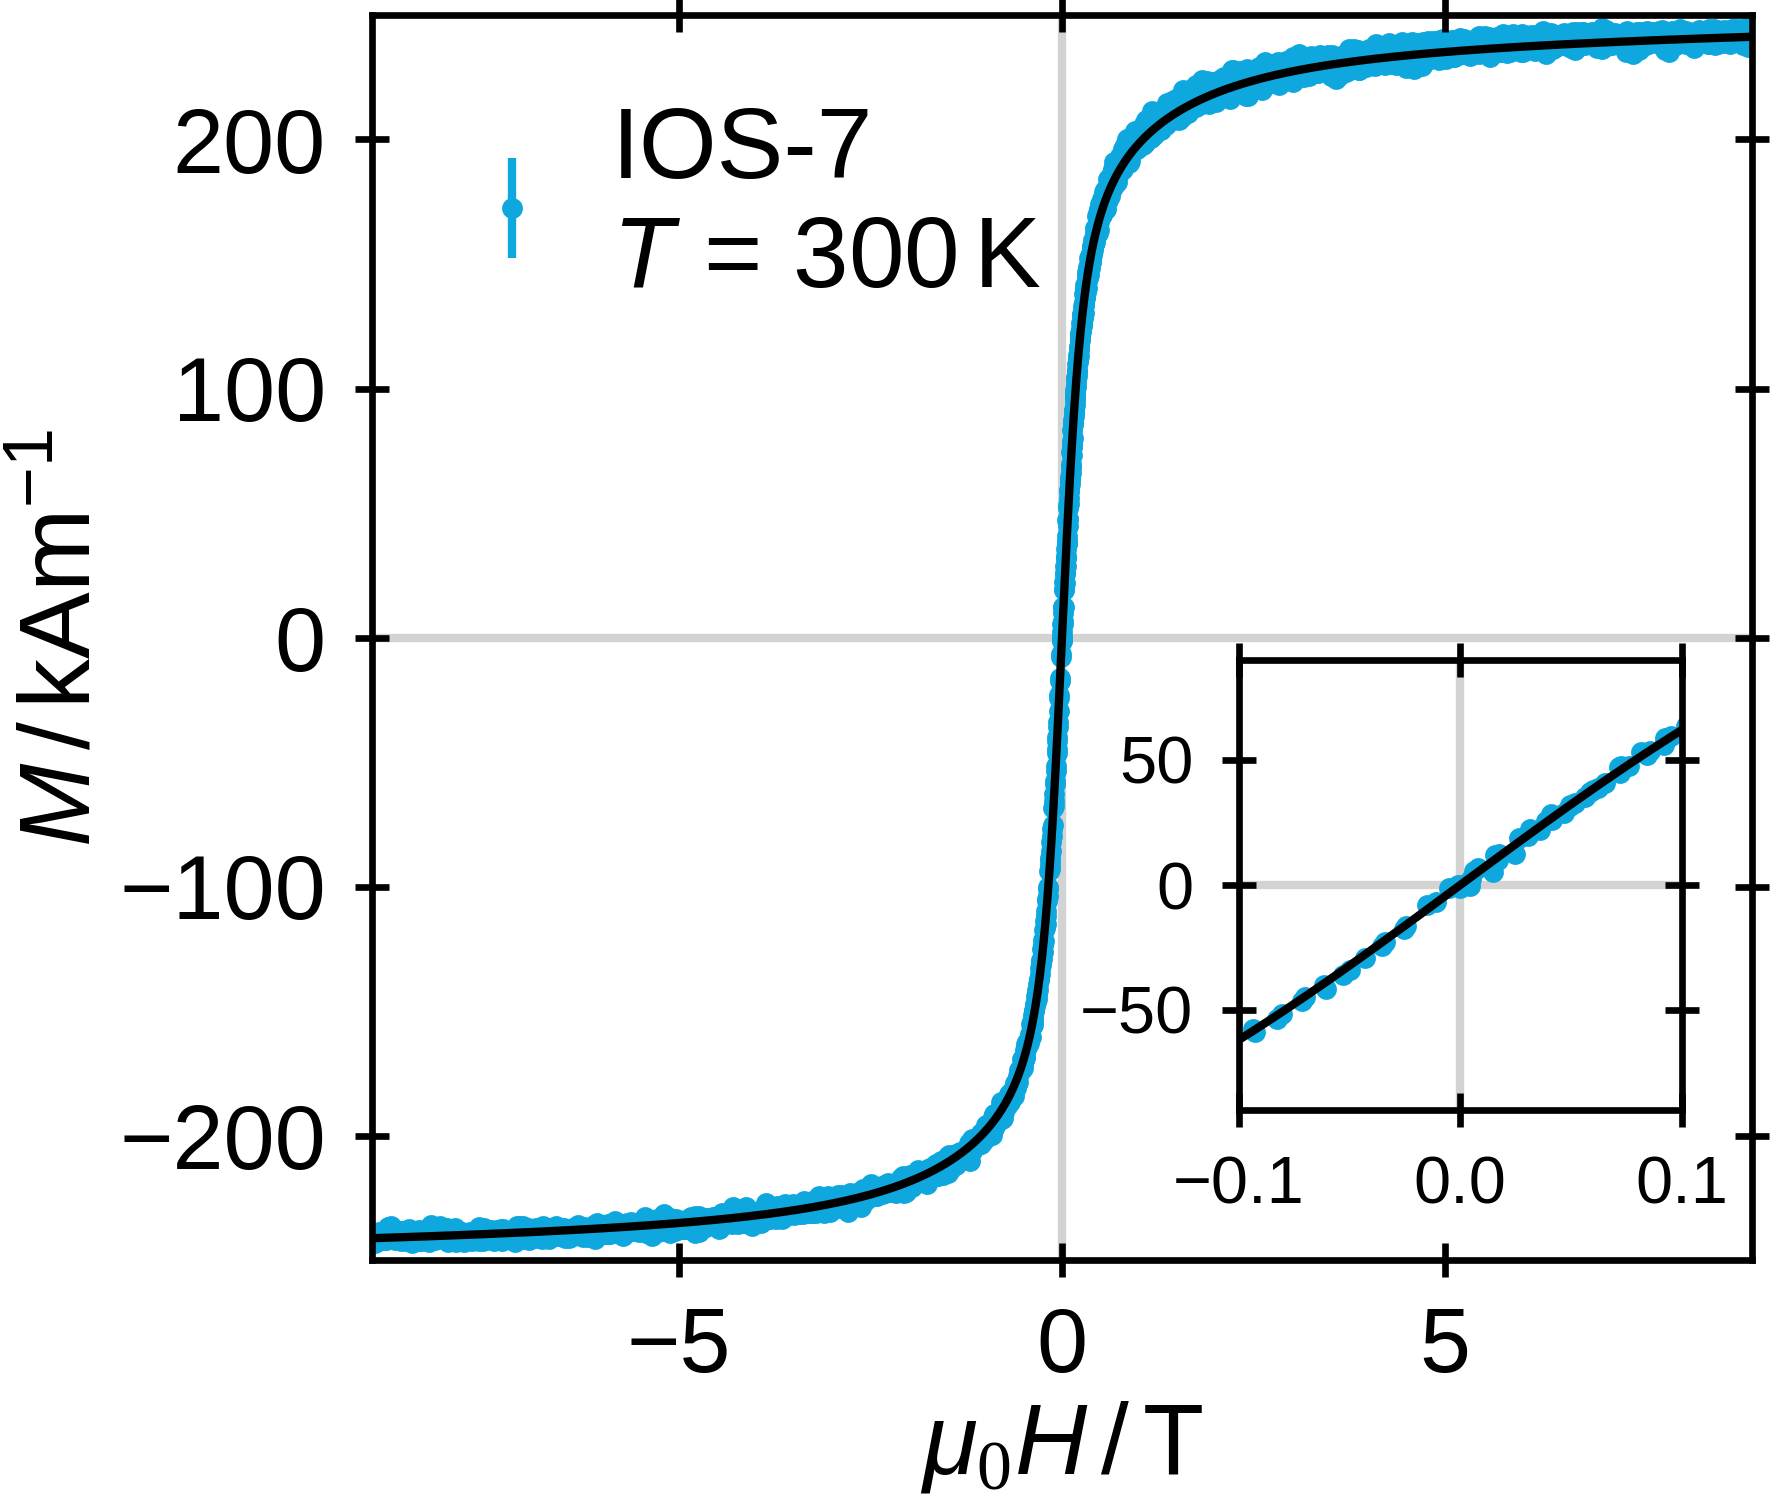
\includegraphics{looselyPackedNP_VSM_IOS-7}
    \caption{\label{fig:looselyPackedNP:nanoparticle:vsm}Room temperature vibrating sample magnetometry for IOS-11 (left) and IOS-7 (right).}
  \end{figure}


  \begin{table}[tb]
    \centering
    \caption{\label{tab:looselyPackedNP:nanoparticle:vsmSanspol}Parameters for the magnetic structure of the nanospheres obtained from VSM and SANSPOL.}
    \begin{tabular}{ c | l | l }
        & IOS-11 & IOS-7 \\
      \hline
      \multicolumn{3}{c}{VSM}\\
      \hline
      $M_s$
        & $153.0(2) \unit{kAm^{-1}}$
        & $168.0(1) \unit{kAm^{-1}}$\\
      $\mu$
        & $12750(30) \, \mu_B$
        & $3770(40) \, \mu_B$\\
      $\chi$
        & $11.8(2) \mu_0$
        & $10.2(9) \mu_0$\\
      \hline
      $r_m$
        & $5.69(2) \unit{nm}$
        & $3.68(4) \unit{nm}$\\
      \hline
      \multicolumn{3}{c}{SANSPOL}\\
      \hline
      $\rho_\mathrm{mag}$
        & $0.52(3) \unit{10^{-6} \angstrom^{-2}}$
        & $0.33(2) \unit{10^{-6} \angstrom^{-2}}$\\
      $d_\mathrm{dead}$
        & $0.3(1) \unit{nm}$
        & $0 \unit{nm}$\\
      \hline
      $M$
        & $179(10) \unit{kAm^{-1}}$
        & $112(9) \unit{kAm^{-1}}$\\
      \hline
    \end{tabular}
  \end{table}

  While being in the same order of magnitude, the determined saturation magnetizations from SANSPOL and VSM are not consistent within the error bars for both samples.
  This can mostly be attributed to the uncertainty introduced into the VSM data when scaling it to the magnetic volume content.
  By estimating the magnetic volume from the magnetic moment and saturation magnetization by
  \begin{align}
    V_p^\mathrm{mag} \eq \frac{\mu}{M_s},
  \end{align}
  a magnetic radius is obtained by
  \begin{align}
    r_m \eq \sqrt[3]{\frac{3 V_p}{4 \pi}}.
  \end{align}
  This is in both cases slightly bigger than the physical particle size, which suggests a small under-estimation of the saturation magnetization in VSM.
  The deviation between the magnetic radius estimated from VSM and physical radius from small-angle scattering is still within the size distribution.
  For the determination of the magnetization from polarized neutron scattering, the splitting of the the two polarization channels is very small for IOS-7 due to the small particle size
  Therefore estimating the parameter for the magnetic scattering length density is limited by the statistical noise, which explains the large deviation of the best fit parameter to the other obtained results.


  %   \begin{figure}[tb]
  %     \centering
  %     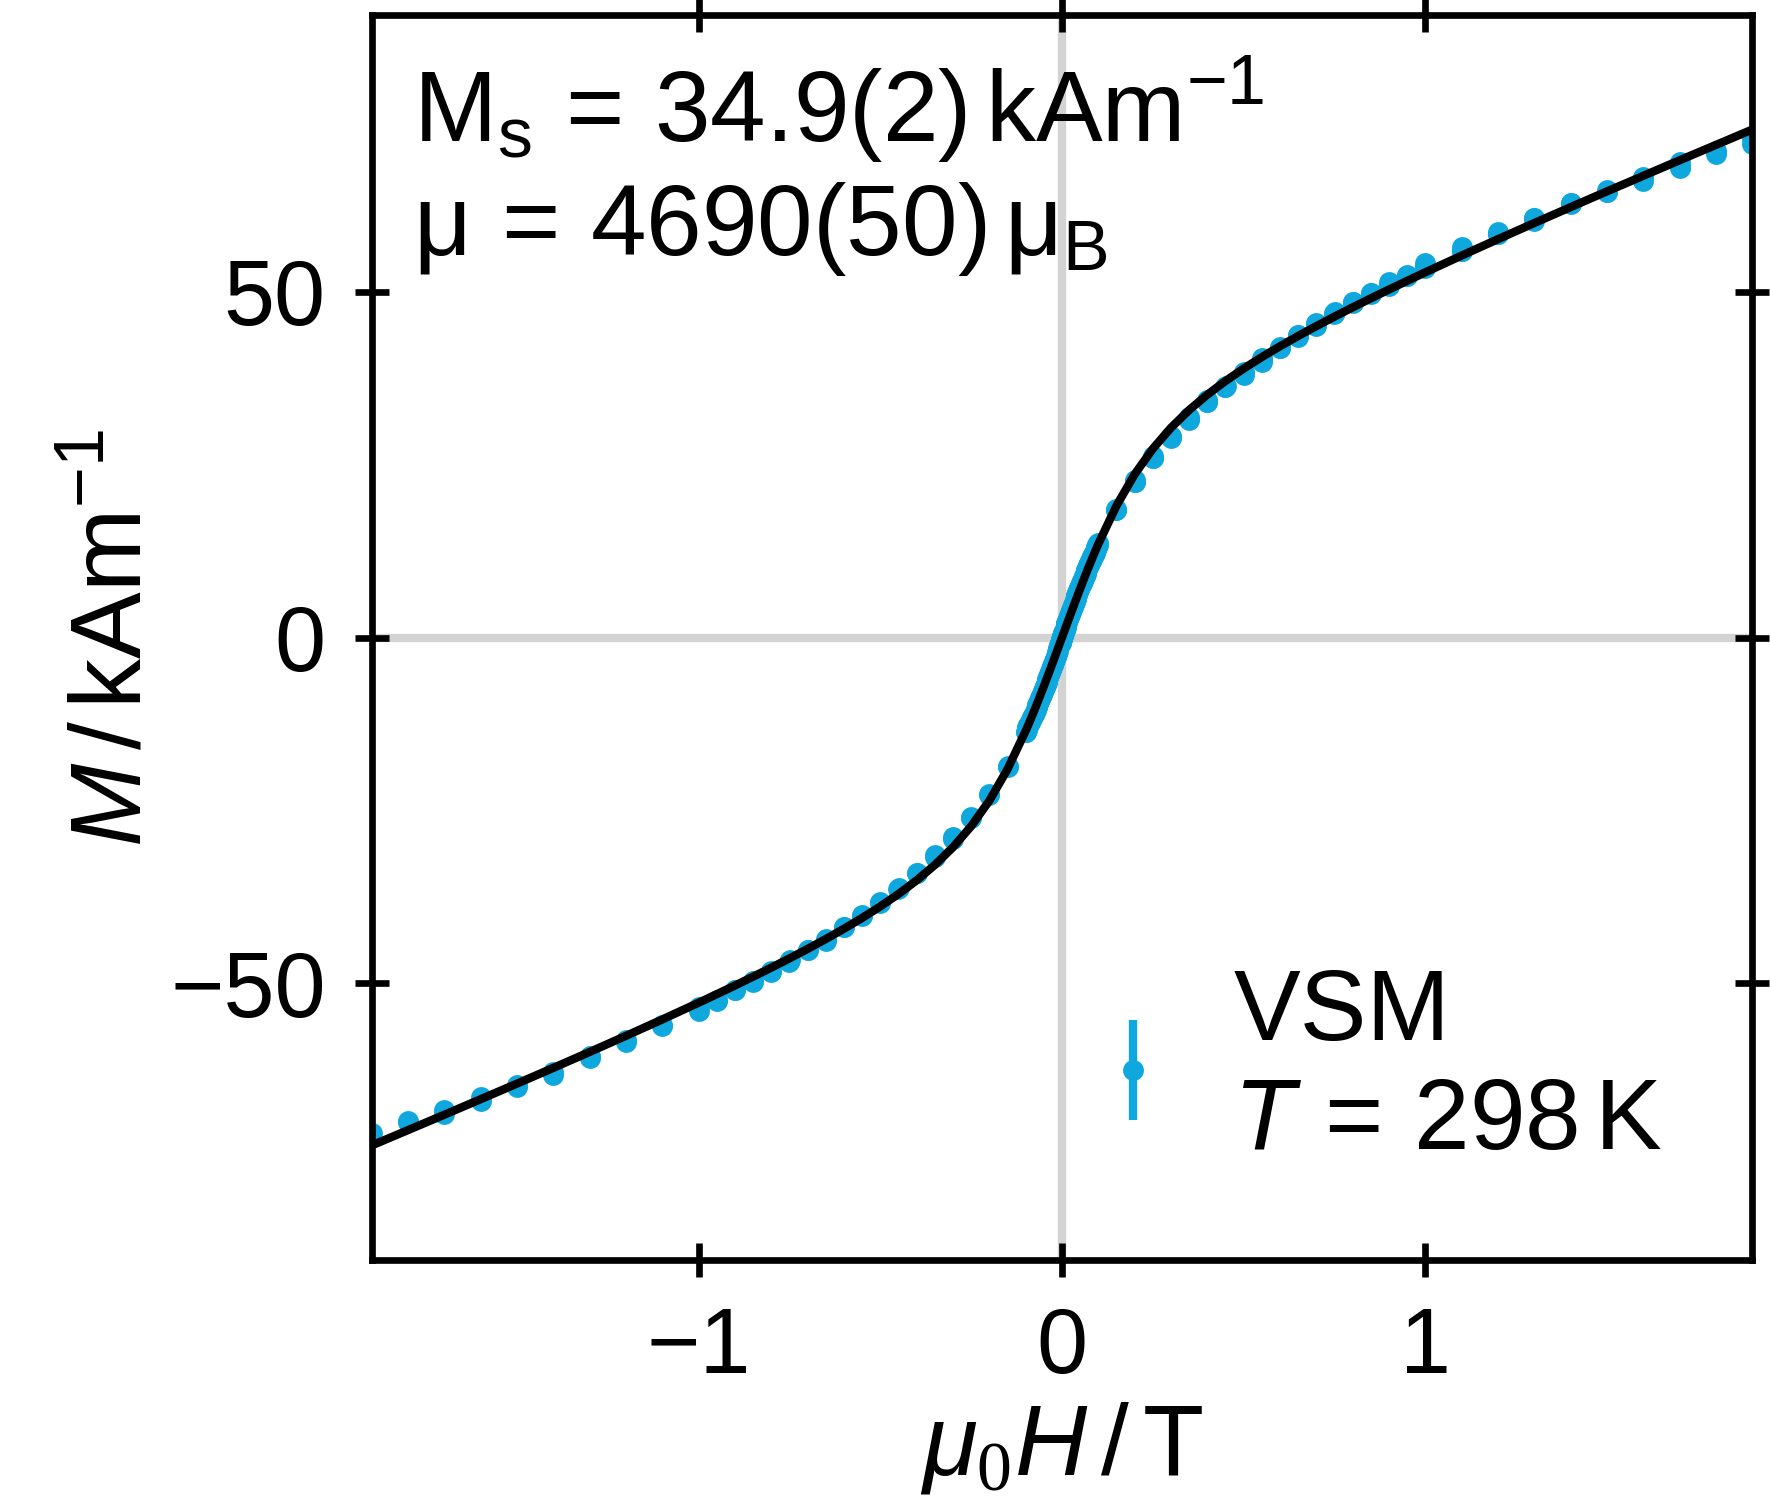
\includegraphics{monolayer_VSM_Ol_CoFe_C}
  %     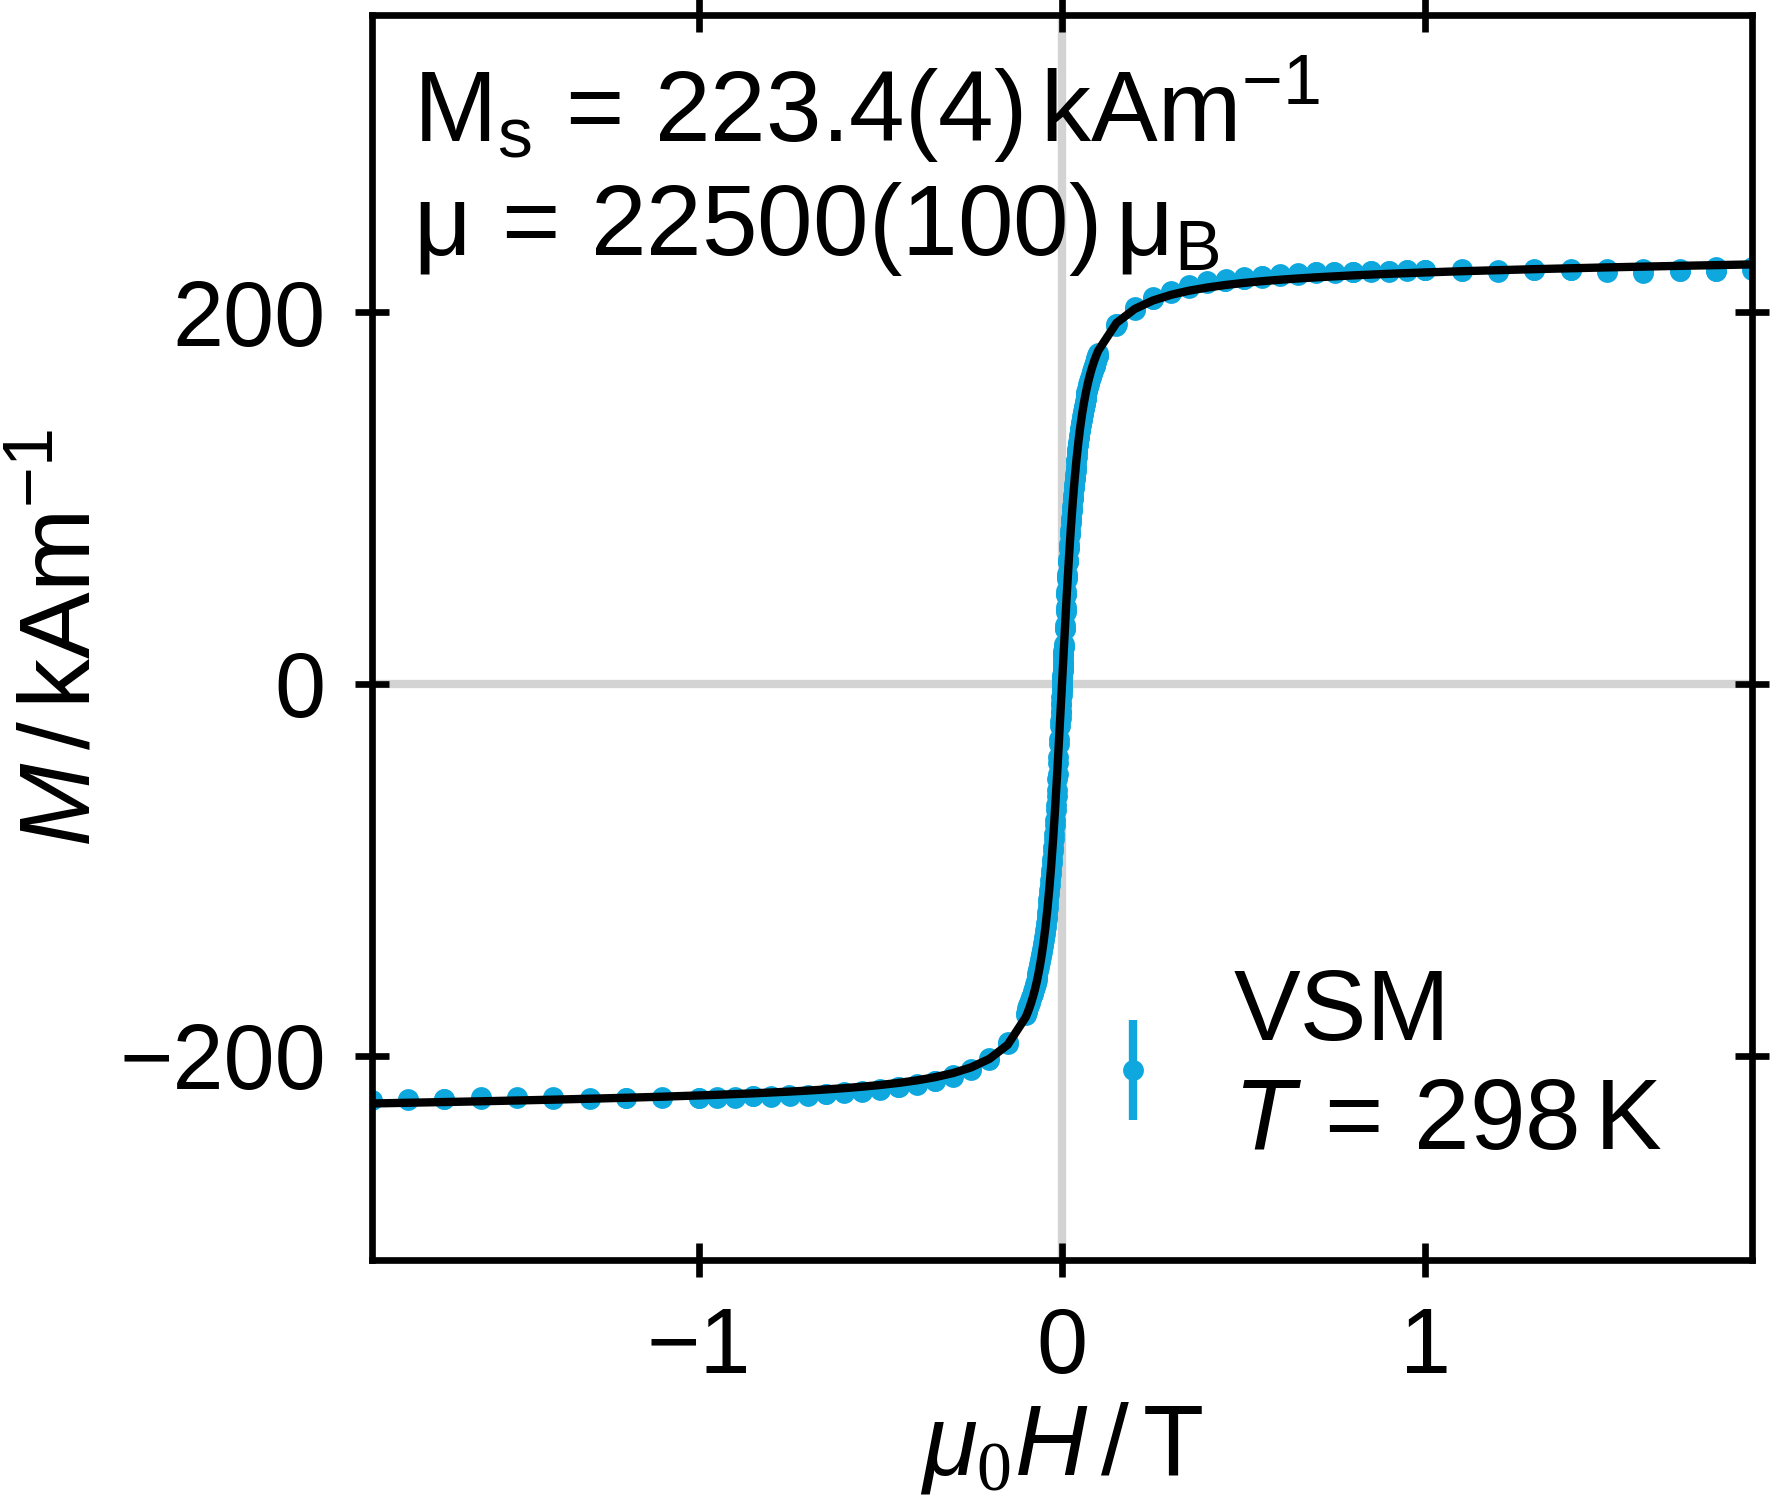
\includegraphics{monolayer_VSM_Ac_CoFe_C}
  %     \caption{\label{fig:monolayers:nanoparticle:vsm}Room-temperature VSM data of Ol-CoFe-C (upper left) and Ac-CoFe-C (lower left) dried on a substrate and fitted to a Langevin curve.}
  %   \end{figure}

  %   This can be compared to the magnetization obtained from measuring the nanoparticles on a vibrating sample magnetometer (VSM) as shown in \reffig{fig:monolayers:nanoparticle:vsm}, which results in magnetizations of $57 \unit{kAm^{-1}}$ for Ol-CoFe-C and $149 \unit{kAm^{-1}}$ for Ac-CoFe-C at the same magnetic field of $1.2 \unit{T}$.

  %   Both experiments agree in the result that the nanoparticles from the oleate route are weakly magnetic, while the particles from the acetylacetonates are stronger magnetic.

  % \paragraphNewLine{Temperature-Dependant VSM}
  % \begin{figure}[tb]
  %   \centering
  %   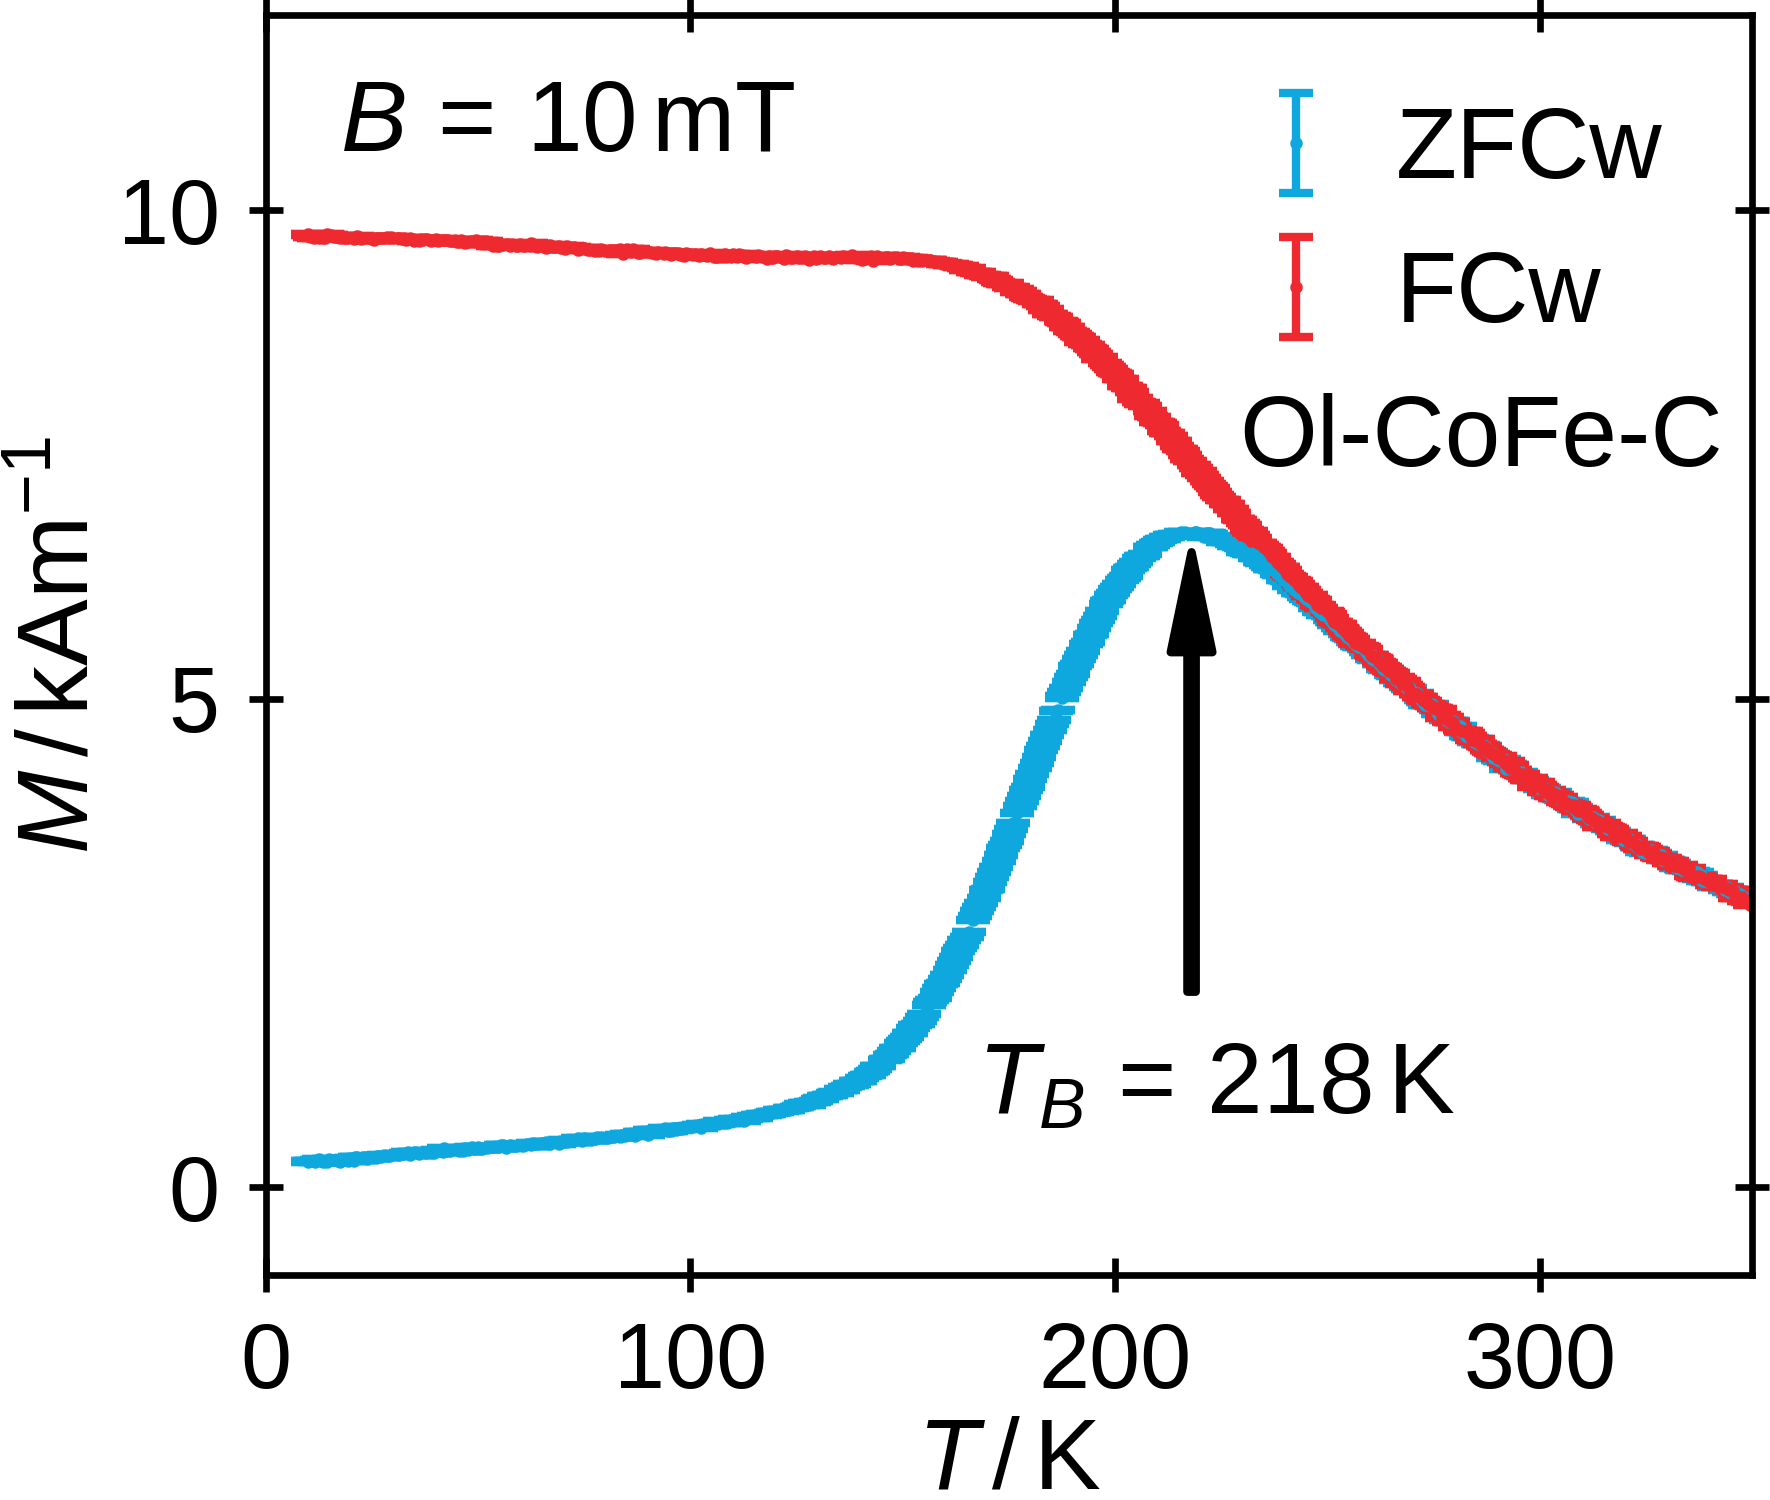
\includegraphics{monolayer_PPMS_ZFC_FC_ML_Ol_CoFe_C}
  %   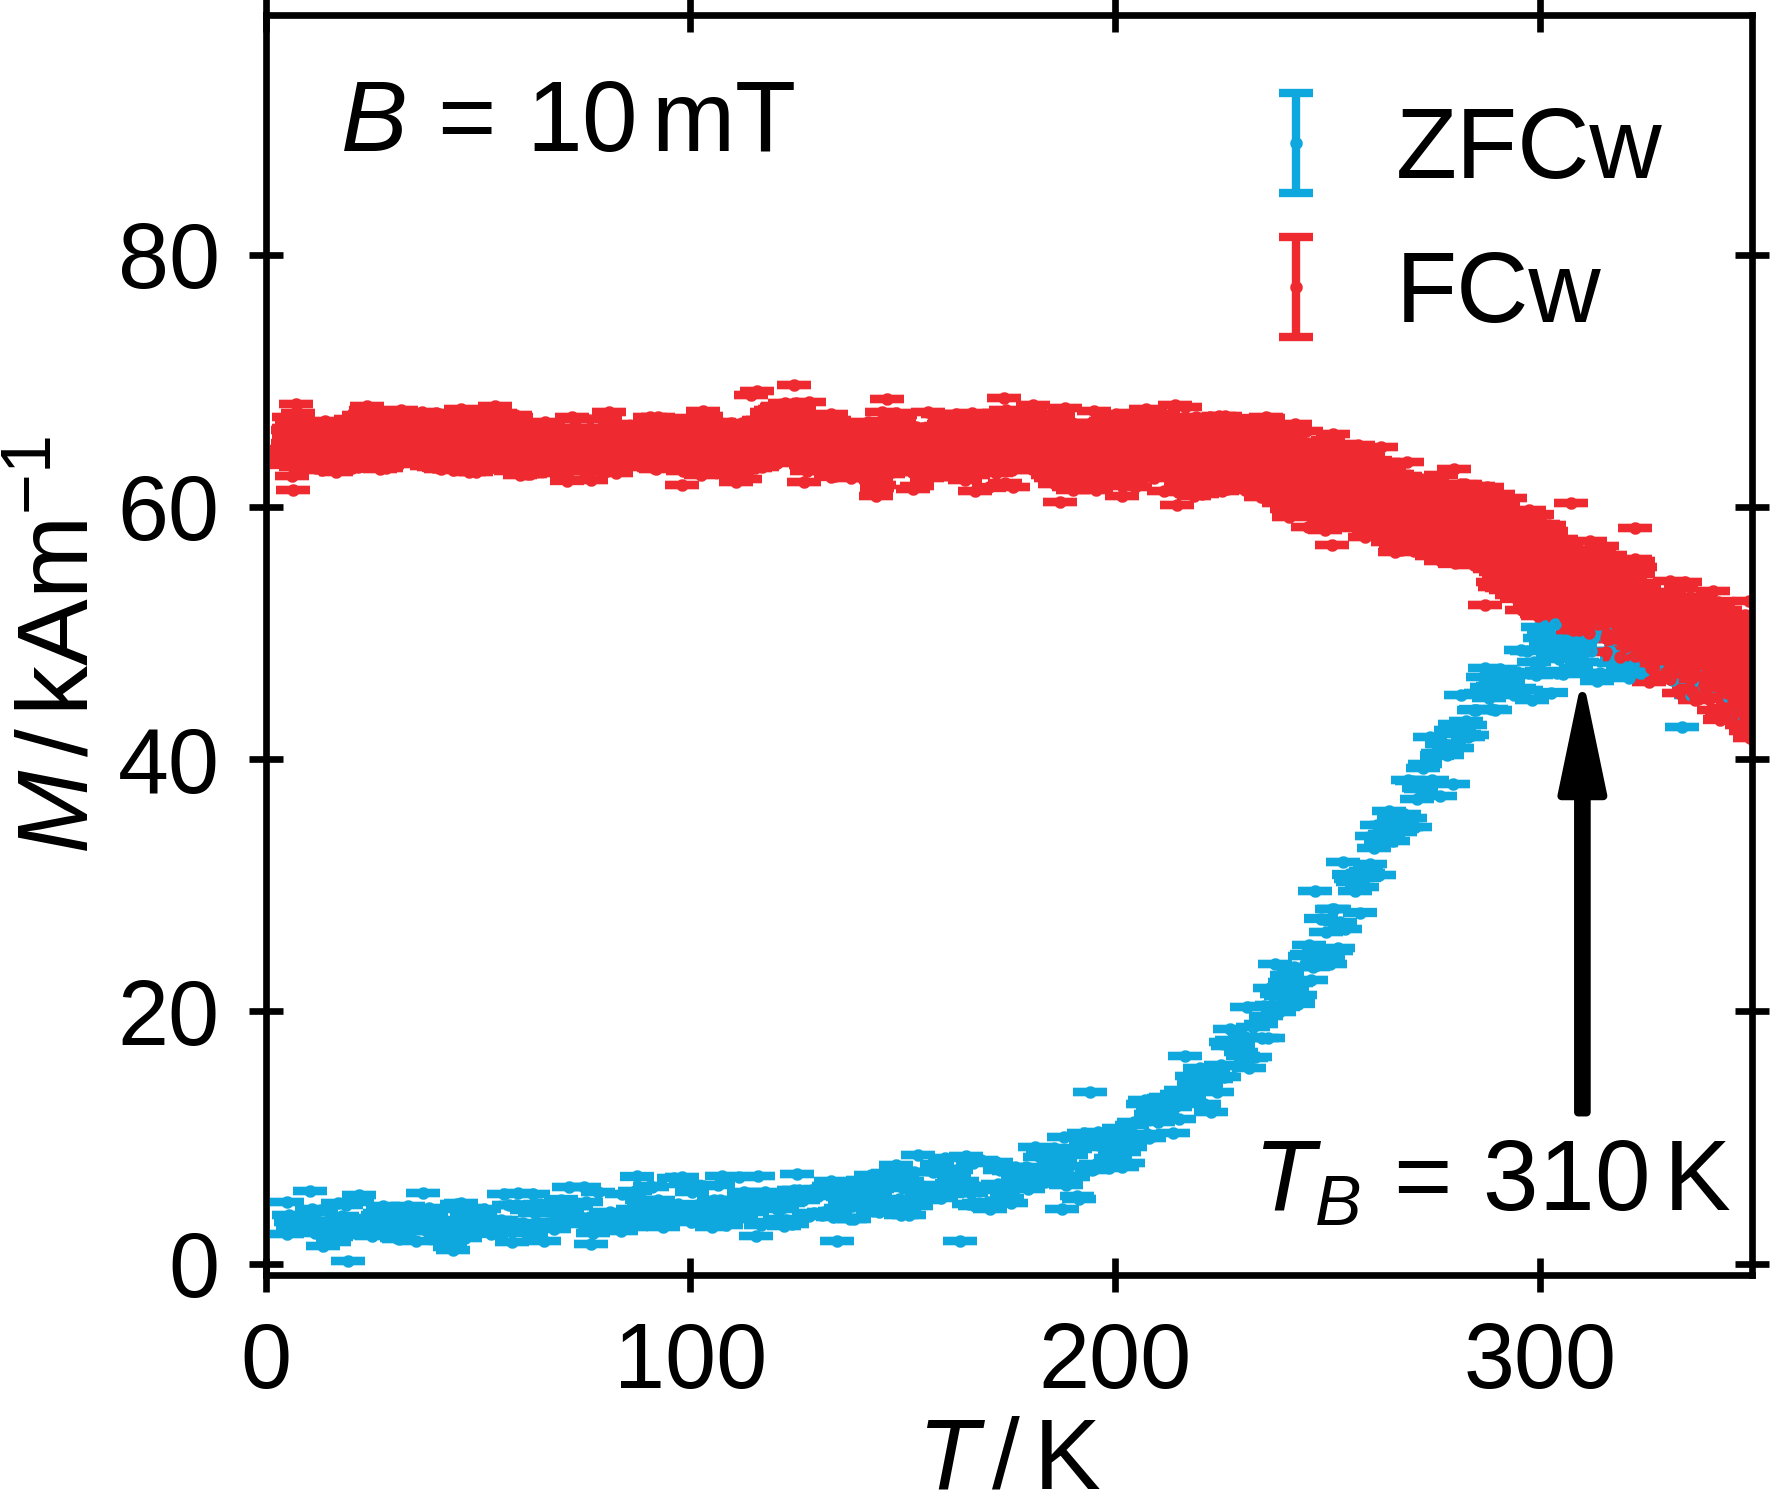
\includegraphics{monolayer_PPMS_ZFC_FC_ML_Ac_CoFe_C}
  %   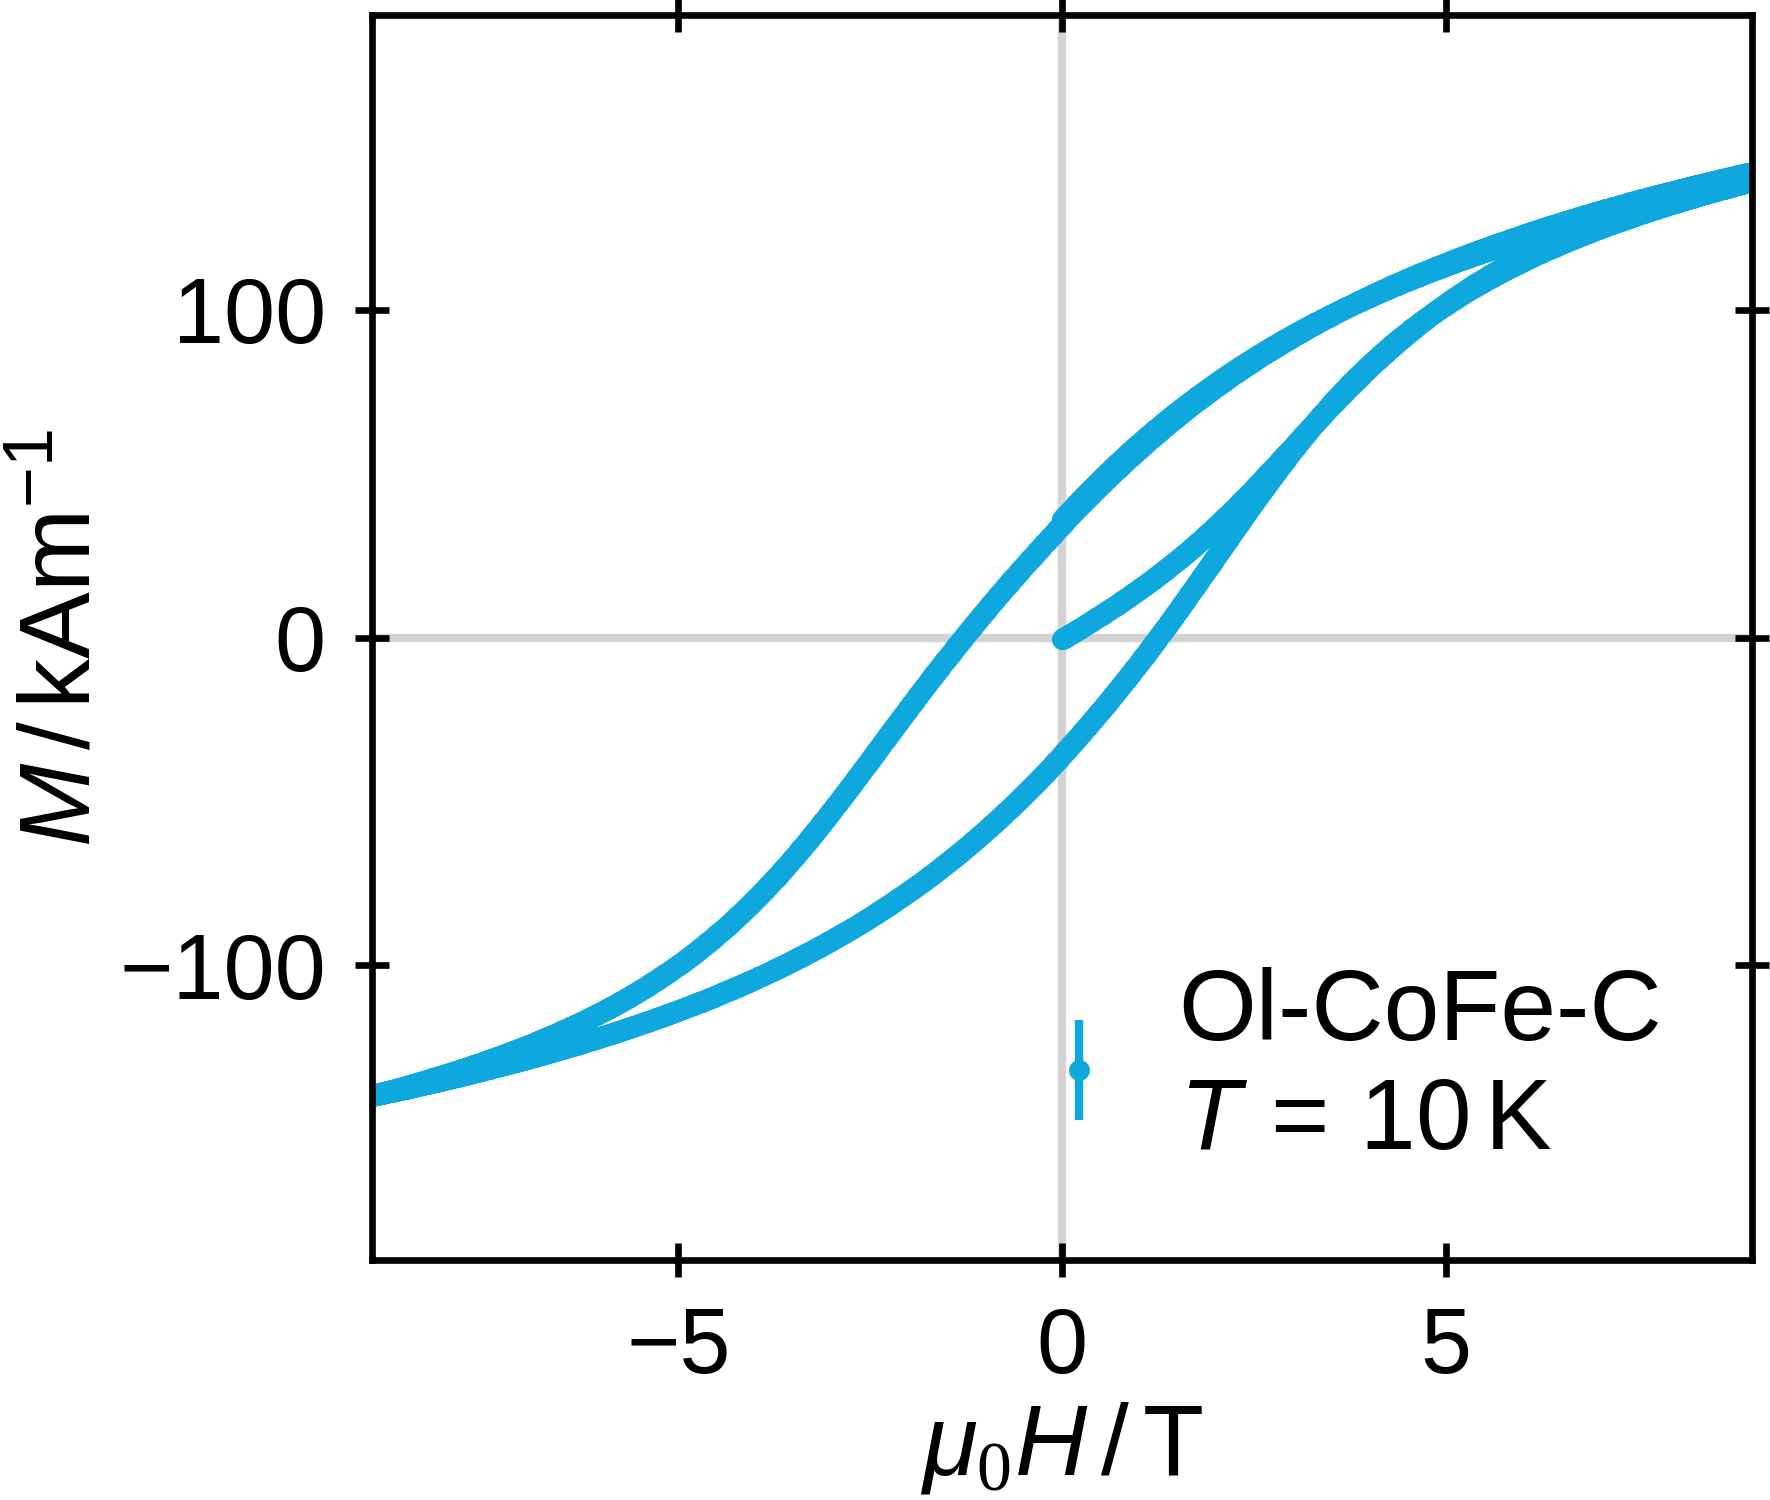
\includegraphics{monolayer_VSM_10K_Ol_CoFe_C}
  %   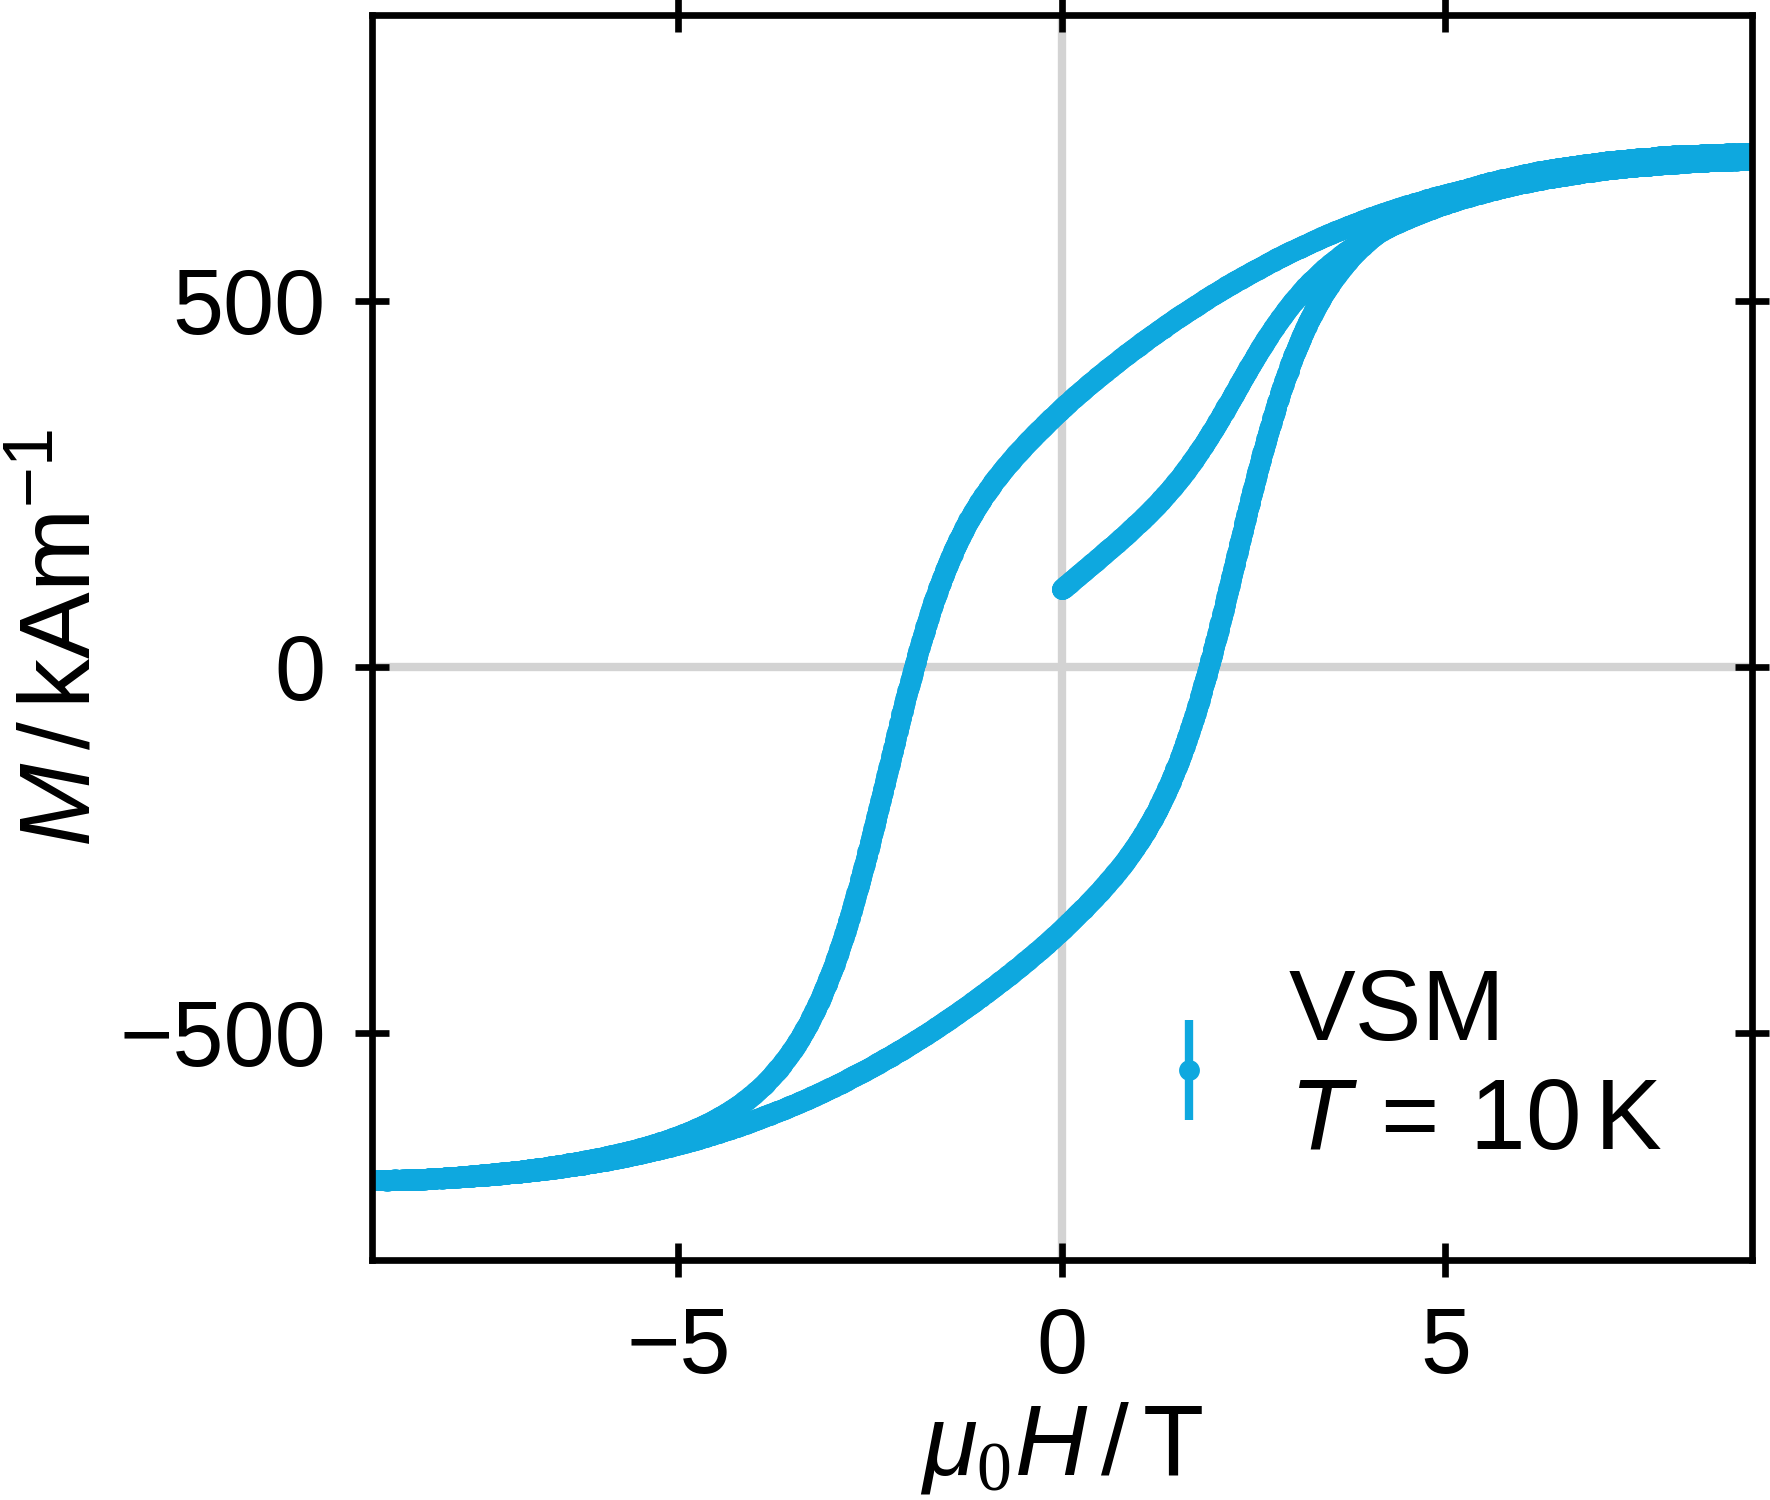
\includegraphics{monolayer_VSM_10K_Ac_CoFe_C}
  %   \caption{\label{fig:monolaye rs:nanoparticle:vsm10K}Low temperature hysteresis measurement of frozen Ol-CoFe-C (left) and Ac-CoFe-C (right) using the same samples as in \reffig{fig:monolayers:nanoparticle:vsm}.}
  % \end{figure}
\end{document}